% !TeX root = Template Latex - Apresentacao - IFSP - SBV.tex

\section{Introduction}
\begin{frame}{Motivation}
    \begin{columns}[c]
    
        \begin{column}{0.6\linewidth}
            \begin{itemize}
                \item Generalize the vector field strategy in \citet{Rezende2022} to allow more motion possibilities, including rotations;
                \item Gain deeper insight into vector field properties through generalization;
                \item Facilitate path following for systems with both translational and rotational motion, such as omnidirectional UAVs and robotic manipulators.
            \end{itemize}
        \end{column}

        \begin{column}{0.4\linewidth}
 
            \begin{figure}
                \centering
                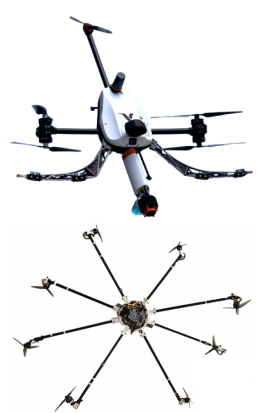
\includegraphics[width=.8\linewidth]{../figures/voliro_omni_vertical.png}
            \end{figure}

        \end{column}

    \end{columns}
    
\end{frame}

\begin{frame}{Contributions}
    \begin{itemize}
        \item Development of a novel vector field guidance strategy applicable to systems with an inherent matrix Lie group structure;
        \item Implementation framework for $\text{SE}(3)$ systems, providing all necessary tools for practical application of the proposed strategy;
        \item Validation through kinematic simulations in $\text{SE}(3)$ and $\text{SO}^+(3,1)$, demonstrating the theoretical results and their practical implications;
        \item Design of an adaptive control strategy for collaborative simulations in $\mathbb{R}^3 \times \text{SO}(3)$, where the vector field guidance strategy generates reference velocities for dynamic control.
    \end{itemize}
\end{frame}

\begin{frame}{Background}
    \begin{tikzpicture}
        % Nodes
        \node (coursework) [block] {Coursework \& assignments};
        \node (culbertson) [block, right of=coursework, xshift=4cm] {Adapt \citet{Culbertson2021} to  vector field of \citet{Rezende2022}};
        % \node (rezende) [block, right of=culbertson, xshift=4cm] {Adaptation to \\ \citet{Rezende2022}};
        \node (pessoa) [block, right of=culbertson, xshift=4cm] {Include orientation \\ $\mathbb{R}^3 \times \text{SO}(3)$  \citep{Pessoa2024}};
        % \node (pessoa) [block, below of=rezende, yshift=-2cm] {Extension to \\ $\mathbb{R}^3 \times \text{SO}(3)$ \\ \citet{Pessoa2024}};
        \node (generalization) [block, below of=pessoa, yshift=-2cm] {Insights into\\ deeper properties};
        % \node (generalization) [block, left of=pessoa, xshift=-4cm] {Generalization to \\ Matrix Lie Groups};
        \node (automatica) [block, left of=generalization, xshift=-4cm] {Generalization to Matrix Lie Groups\\ (\textit{Automatica} submission)};
    
        % Arrows
        \draw [arrow] (coursework) -- (culbertson);
        \draw [arrow] (culbertson) -- (pessoa);
        % \draw [arrow] (rezende) -- (pessoa);
        \draw [arrow] (pessoa) -- (generalization);
        \draw [arrow] (generalization) -- (automatica);
    \end{tikzpicture}
\end{frame}

% \begin{frame}

%     \frametitle{Motivação}
%      Incorporar orientação ao campo de \citet{Rezende2022}, adotando o modelo:
%      \begin{align*}
%          \boldsymbol{\xi} = \begin{bmatrix}
%              \dot{\mathbf{p}} \\ \boldsymbol{\omega}
%          \end{bmatrix} = \begin{bmatrix}
%              \dot{\mathbf{p}}_d \\ \boldsymbol{\omega}_d \end{bmatrix}.
%      \end{align*}

%      Exemplos de aplicação:
%     \begin{itemize}
%        	\item Controle de um VANT omnidirecional para circular uma curva com orientações predefinidas.
%         \item Manipulação de um objeto grande, que deve seguir uma sequência específica de posições e orientações durante o transporte.
%     \end{itemize}
%     % \vspace{0.5cm}
% \end{frame}